\documentclass[14pt]{extbook}
\usepackage{multicol, enumerate, enumitem, hyperref, color, soul, setspace, parskip, fancyhdr} %General Packages
\usepackage{amssymb, amsthm, amsmath, bbm, latexsym, units, mathtools} %Math Packages
\everymath{\displaystyle} %All math in Display Style
% Packages with additional options
\usepackage[headsep=0.5cm,headheight=12pt, left=1 in,right= 1 in,top= 1 in,bottom= 1 in]{geometry}
\usepackage[usenames,dvipsnames]{xcolor}
\usepackage{dashrule}  % Package to use the command below to create lines between items
\newcommand{\litem}[1]{\item#1\hspace*{-1cm}\rule{\textwidth}{0.4pt}}
\pagestyle{fancy}
\lhead{Progress Quiz 8}
\chead{}
\rhead{Version A}
\lfoot{4553-3922}
\cfoot{}
\rfoot{Fall 2020}
\begin{document}

\begin{enumerate}
\litem{
Solve the radical equation below. Then, choose the interval(s) that the solution(s) belongs to.\[ \sqrt{-9 x + 5} - \sqrt{4 x - 6} = 0 \]\begin{enumerate}[label=\Alph*.]
\item \( x_1 \in [0.48, 0.62] \text{ and } x_2 \in [0.8,1.1] \)
\item \( x_1 \in [0.48, 0.62] \text{ and } x_2 \in [1.37,1.67] \)
\item \( x \in [-0.39,-0.03] \)
\item \( \text{All solutions lead to invalid or complex values in the equation.} \)
\item \( x \in [0.83,0.86] \)

\end{enumerate} }
\litem{
What is the domain of the function below?\[ f(x) = \sqrt[4]{-4 x + 7} \]\begin{enumerate}[label=\Alph*.]
\item \( (-\infty, a], \text{where } a \in [-0.5, 1.47] \)
\item \( [a, \infty), \text{where } a \in [1.3, 2.6] \)
\item \( [a, \infty), \text{where } a \in [-3, 1.4] \)
\item \( (-\infty, \infty) \)
\item \( (-\infty, a], \text{ where } a \in [1.58, 3.33] \)

\end{enumerate} }
\litem{
Solve the radical equation below. Then, choose the interval(s) that the solution(s) belongs to.\[ \sqrt{42 x^2 + 48} - \sqrt{-90 x} = 0 \]\begin{enumerate}[label=\Alph*.]
\item \( \text{All solutions lead to invalid or complex values in the equation.} \)
\item \( x \in [-1.28,-1.03] \)
\item \( x_1 \in [-1.28, -1.03] \text{ and } x_2 \in [-2,1] \)
\item \( x_1 \in [0.66, 1.88] \text{ and } x_2 \in [1.14,3.14] \)
\item \( x \in [-1.01,-0.68] \)

\end{enumerate} }
\litem{
Solve the radical equation below. Then, choose the interval(s) that the solution(s) belongs to.\[ \sqrt{48 x^2 + 6} - \sqrt{-34 x} = 0 \]\begin{enumerate}[label=\Alph*.]
\item \( x_1 \in [0.33, 0.39] \text{ and } x_2 \in [0.27,1.33] \)
\item \( \text{All solutions lead to invalid or complex values in the equation.} \)
\item \( x \in [-0.36,-0.3] \)
\item \( x_1 \in [-0.4, -0.36] \text{ and } x_2 \in [-1.21,-0.28] \)
\item \( x \in [-0.4,-0.36] \)

\end{enumerate} }
\litem{
Choose the graph of the equation below.\[ f(x) = - \sqrt{x - 10} - 5 \]\begin{enumerate}[label=\Alph*.]
\begin{multicols}{2}\item 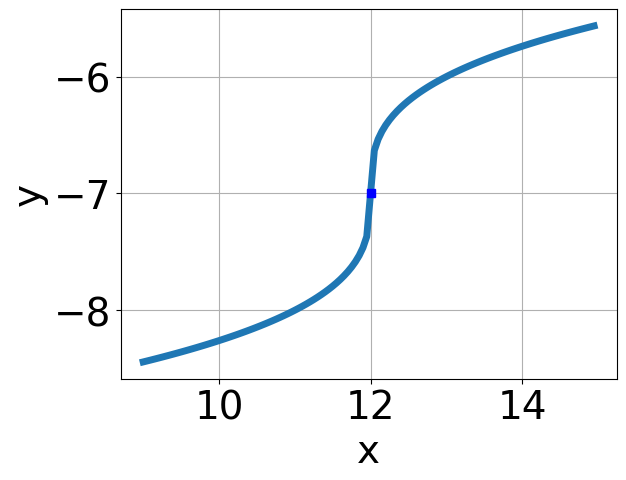
\includegraphics[width = 0.3\textwidth]{../Figures/radicalEquationToGraphAA.png}\item 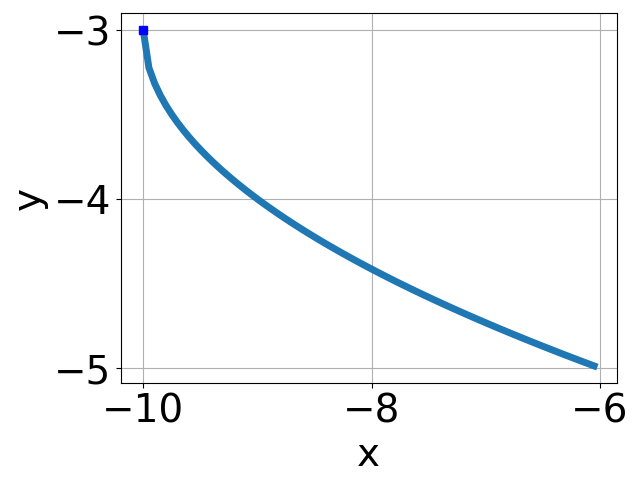
\includegraphics[width = 0.3\textwidth]{../Figures/radicalEquationToGraphBA.png}\item 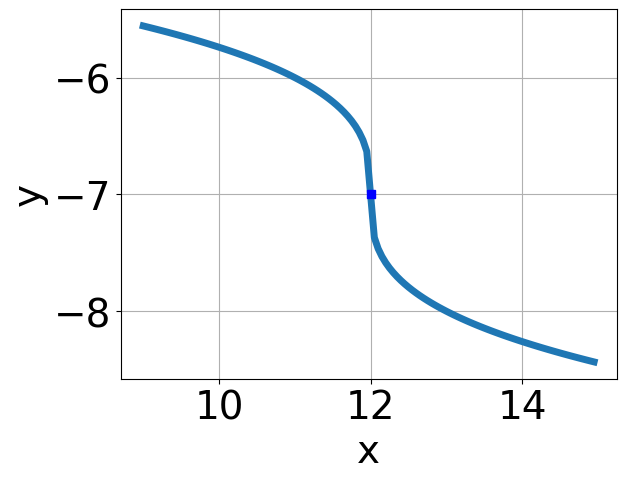
\includegraphics[width = 0.3\textwidth]{../Figures/radicalEquationToGraphCA.png}\item 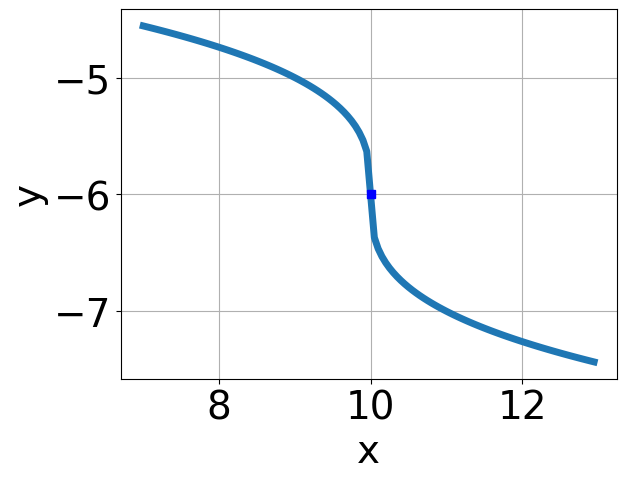
\includegraphics[width = 0.3\textwidth]{../Figures/radicalEquationToGraphDA.png}\end{multicols}\item None of the above.
\end{enumerate} }
\litem{
Choose the equation of the function graphed below.
\begin{center}
    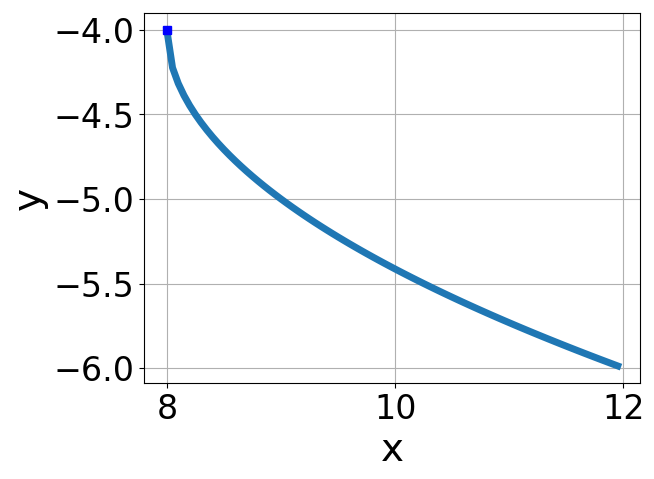
\includegraphics[width=0.5\textwidth]{../Figures/radicalGraphToEquationA.png}
\end{center}
\begin{enumerate}[label=\Alph*.]
\item \( f(x) = \sqrt[3]{x - 8} - 3 \)
\item \( f(x) = \sqrt[3]{x + 8} - 3 \)
\item \( f(x) = - \sqrt[3]{x - 8} - 3 \)
\item \( f(x) = - \sqrt[3]{x + 8} - 3 \)
\item \( \text{None of the above} \)

\end{enumerate} }
\litem{
Solve the radical equation below. Then, choose the interval(s) that the solution(s) belongs to.\[ \sqrt{5 x - 7} - \sqrt{3 x + 8} = 0 \]\begin{enumerate}[label=\Alph*.]
\item \( x \in [-2.5,1.2] \)
\item \( \text{All solutions lead to invalid or complex values in the equation.} \)
\item \( x_1 \in [-3.3, -2.5] \text{ and } x_2 \in [1.4,3.4] \)
\item \( x \in [6.1,8.3] \)
\item \( x_1 \in [0.6, 1.6] \text{ and } x_2 \in [6.5,8.5] \)

\end{enumerate} }
\litem{
Choose the equation of the function graphed below.
\begin{center}
    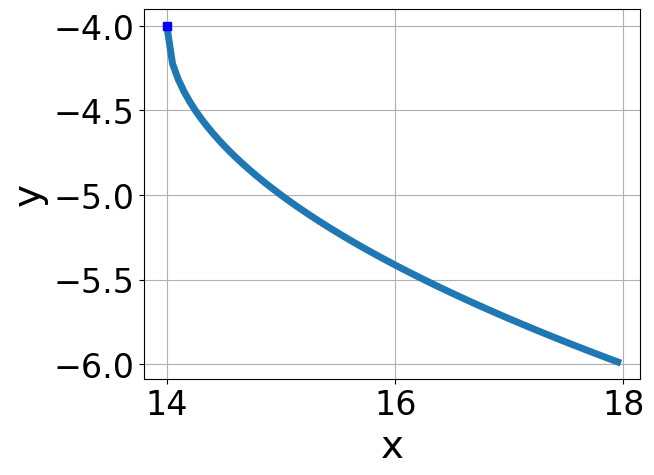
\includegraphics[width=0.5\textwidth]{../Figures/radicalGraphToEquationCopyA.png}
\end{center}
\begin{enumerate}[label=\Alph*.]
\item \( f(x) = - \sqrt[3]{x - 6} - 7 \)
\item \( f(x) = \sqrt[3]{x - 6} - 7 \)
\item \( f(x) = \sqrt[3]{x + 6} - 7 \)
\item \( f(x) = - \sqrt[3]{x + 6} - 7 \)
\item \( \text{None of the above} \)

\end{enumerate} }
\litem{
Choose the graph of the equation below.\[ f(x) = \sqrt{x + 8} + 6 \]\begin{enumerate}[label=\Alph*.]
\begin{multicols}{2}\item 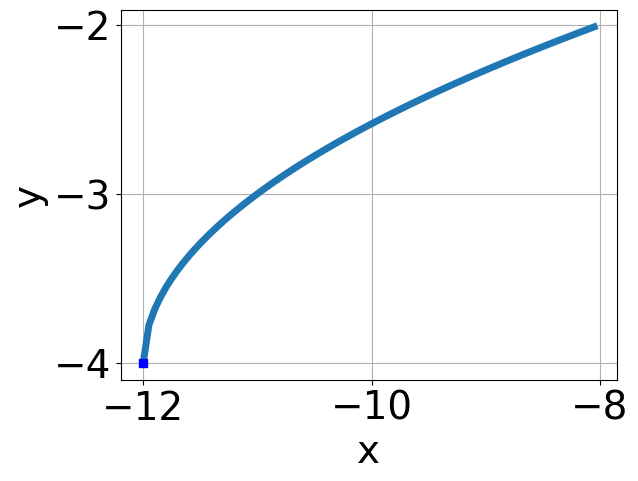
\includegraphics[width = 0.3\textwidth]{../Figures/radicalEquationToGraphCopyAA.png}\item 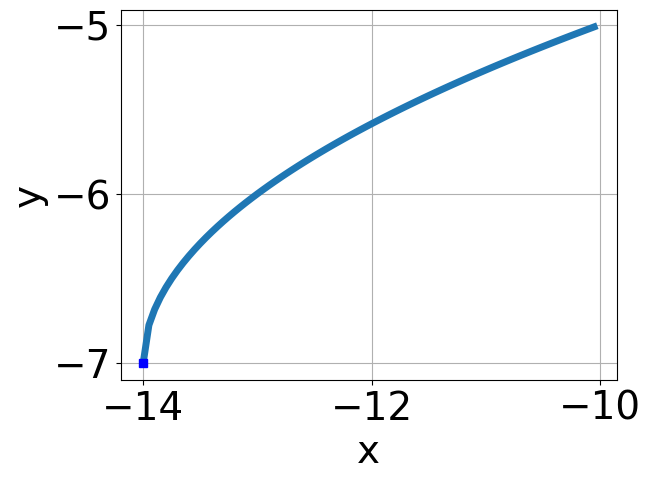
\includegraphics[width = 0.3\textwidth]{../Figures/radicalEquationToGraphCopyBA.png}\item 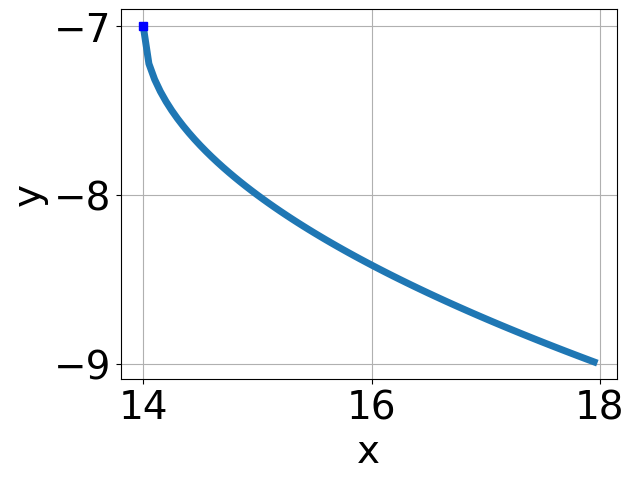
\includegraphics[width = 0.3\textwidth]{../Figures/radicalEquationToGraphCopyCA.png}\item 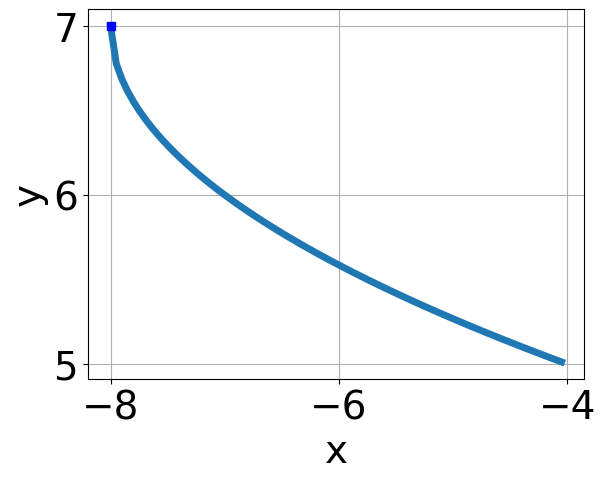
\includegraphics[width = 0.3\textwidth]{../Figures/radicalEquationToGraphCopyDA.png}\end{multicols}\item None of the above.
\end{enumerate} }
\litem{
What is the domain of the function below?\[ f(x) = \sqrt[4]{-4 x + 5} \]\begin{enumerate}[label=\Alph*.]
\item \( [a, \infty), \text{where } a \in [1.12, 1.45] \)
\item \( (-\infty, a], \text{where } a \in [0.46, 1.16] \)
\item \( [a, \infty), \text{where } a \in [0.26, 0.81] \)
\item \( (-\infty, a], \text{ where } a \in [0.84, 1.44] \)
\item \( (-\infty, \infty) \)

\end{enumerate} }
\end{enumerate}

\end{document}